\documentclass{sigchi}

% Use this section to set the ACM copyright statement (e.g. for
% preprints).  Consult the conference website for the camera-ready
% copyright statement.

% Copyright
\CopyrightYear{2019}
%\setcopyright{acmcopyright}
\setcopyright{acmlicensed}
%\setcopyright{rightsretained}
%\setcopyright{usgov}
%\setcopyright{usgovmixed}
%\setcopyright{cagov}
%\setcopyright{cagovmixed}
% DOI
\doi{http://dx.doi.org/10.475/123_4}
% ISBN
\isbn{123-4567-24-567/08/06}
%Conference
\conferenceinfo{L@S'19,}{June 24--25, 2019, Chicago, CA, USA}
%Price
\acmPrice{\$15.00}

% Use this command to override the default ACM copyright statement
% (e.g. for preprints).  Consult the conference website for the
% camera-ready copyright statement.

%% HOW TO OVERRIDE THE DEFAULT COPYRIGHT STRIP --
%% Please note you need to make sure the copy for your specific
%% license is used here!
% \toappear{
% Permission to make digital or hard copies of all or part of this work
% for personal or classroom use is granted without fee provided that
% copies are not made or distributed for profit or commercial advantage
% and that copies bear this notice and the full citation on the first
% page. Copyrights for components of this work owned by others than ACM
% must be honored. Abstracting with credit is permitted. To copy
% otherwise, or republish, to post on servers or to redistribute to
% lists, requires prior specific permission and/or a fee. Request
% permissions from \href{mailto:Permissions@acm.org}{Permissions@acm.org}. \\
% \emph{CHI '16},  May 07--12, 2016, San Jose, CA, USA \\
% ACM xxx-x-xxxx-xxxx-x/xx/xx\ldots \$15.00 \\
% DOI: \url{http://dx.doi.org/xx.xxxx/xxxxxxx.xxxxxxx}
% }

% Arabic page numbers for submission.  Remove this line to eliminate
% page numbers for the camera ready copy
% \pagenumbering{arabic}

% Load basic packages
\usepackage{balance}       % to better equalize the last page
\usepackage{graphics}      % for EPS, load graphicx instead 
\usepackage[T1]{fontenc}   % for umlauts and other diaeresis
\usepackage{txfonts}
\usepackage{mathptmx}
\usepackage[pdflang={en-US},pdftex]{hyperref}
\usepackage{color}
\usepackage{booktabs}
\usepackage{textcomp}

\usepackage{bbm}
\usepackage{nameref}
\usepackage{listings}

% Some optional stuff you might like/need.
\usepackage{microtype}        % Improved Tracking and Kerning
% \usepackage[all]{hypcap}    % Fixes bug in hyperref caption linking
\usepackage{ccicons}          % Cite your images correctly!
% \usepackage[utf8]{inputenc} % for a UTF8 editor only

% If you want to use todo notes, marginpars etc. during creation of
% your draft document, you have to enable the "chi_draft" option for
% the document class. To do this, change the very first line to:
% "\documentclass[chi_draft]{sigchi}". You can then place todo notes
% by using the "\todo{...}"  command. Make sure to disable the draft
% option again before submitting your final document.
\usepackage{todonotes}

% Paper metadata (use plain text, for PDF inclusion and later
% re-using, if desired).  Use \emtpyauthor when submitting for review
% so you remain anonymous.
\def\plaintitle{Via: Illuminating Academic Pathways at Scale}
\def\plainauthor{First Author, Second Author, Third Author,
  Fourth Author, Fifth Author, Sixth Author}
\def\emptyauthor{}
\def\plainkeywords{Authors' choice; of terms; separated; by
  semicolons; include commas, within terms only; required.}
\def\plaingeneralterms{Documentation, Standardization}

% llt: Define a global style for URLs, rather that the default one
\makeatletter
\def\url@leostyle{%
  \@ifundefined{selectfont}{
    \def\UrlFont{\sf}
  }{
    \def\UrlFont{\small\bf\ttfamily}
  }}
\makeatother
\urlstyle{leo}

% To make various LaTeX processors do the right thing with page size.
\def\pprw{8.5in}
\def\pprh{11in}
\special{papersize=\pprw,\pprh}
\setlength{\paperwidth}{\pprw}
\setlength{\paperheight}{\pprh}
\setlength{\pdfpagewidth}{\pprw}
\setlength{\pdfpageheight}{\pprh}

% Andreas
\setlength{\textfloatsep}{10pt}
\newcommand{\secref}[1]{{\em\nameref{#1}}}

\newcommand{\squishlist}{
  \begin{list}{$\bullet$}
    {
      \setlength{\itemsep}{0pt}
      \setlength{\parsep}{3pt}
      \setlength{\topsep}{3pt}
      \setlength{\partopsep}{0pt}
      \setlength{\leftmargin}{1.5em}
      \setlength{\labelwidth}{1em}
      \setlength{\labelsep}{0.5em}
    }
}

\newcommand{\squishend}{
  \end{list}
}

% Make sure hyperref comes last of your loaded packages, to give it a
% fighting chance of not being over-written, since its job is to
% redefine many LaTeX commands.
\definecolor{linkColor}{RGB}{6,125,233}
\hypersetup{%
  pdftitle={\plaintitle},
% Use \plainauthor for final version.
%  pdfauthor={\plainauthor},
  pdfauthor={\emptyauthor},
  pdfkeywords={\plainkeywords},
  pdfdisplaydoctitle=true, % For Accessibility
  bookmarksnumbered,
  pdfstartview={FitH},
  colorlinks,
  citecolor=black,
  filecolor=black,
  linkcolor=black,
  urlcolor=linkColor,
  breaklinks=true,
  hypertexnames=false
}

% create a shortcut to typeset table headings
% \newcommand\tabhead[1]{\small\textbf{#1}}

% End of preamble. Here it comes the document.
\begin{document}

\title{\plaintitle}

\numberofauthors{4}
\author{%
  \alignauthor{Geoffrey Angus \thanks{Equal Contribution.}\\
    \affaddr{Stanford University}\\
    \affaddr{Stanford, CA}\\
    \email{gangus@stanford.edu}}\\
  \alignauthor{Richard Diehl Martinez \footnotemark[1]\\
    \affaddr{Stanford University}\\
    \affaddr{Stanford, CA}\\
    \email{rdm@stanford.edu}}\\
  \alignauthor{Mitchell L. Stevens\\
    \affaddr{Stanford University}\\
    \affaddr{Stanford, CA}\\
    \email{stevens4@stanford.edu}}\\
  \alignauthor{Andreas Paepcke\\
    \affaddr{Stanford University}\\
    \affaddr{Stanford, CA}\\
    \email{paepcke@cs.stanford.edu}}\\
}

\maketitle

\begin{abstract}
The processes through which course selections accumulate into college
pathways in US higher education is poorly instrumented for observation
at scale. We offer an analytic toolkit, called {\em Via}, which
transforms commonly available enrollment data into formal graphs that
are amenable to interactive visualizations and computational
exploration. We explain the procedures required to project enrollment records onto graphs, and then demonstrate the toolkit utilizing eighteen years of enrollment data at a large private research university. Findings complement prior research on academic search and offer powerful new means for making pathway navigation more efficient.
 \end{abstract}

\category{H.5.m.}{Information Interfaces and Presentation
  (e.g. HCI)}{Miscellaneous}{}{}

\keywords{Course Sequences; Academic Pathways; Graph Visualization}

\section{Introduction}
%%{\color{red}[LOCKED BY ANDREAS]}


%% - What is the problem?
%% - Why is it important?
%% - Why is it hard?
%% - How are current solutions insufficient?
%% - What we do

US higher education is unique in the world in the extent to
which schools expect undergraduates to explore a variety of courses before committing to a field of study. In contrast with virtually all other national postsecondary systems, in which students enter schools and programs with relatively structured curricula, US undergraduates are encouraged to explore a variety of academic options through an iterative course search and selection process. We call a student's
eventual sequence of course elections a {\it pathway}. Pathways are notoriously poorly instrumented for observation by students, educators, administrators or researchers \cite{chambliss2014college}.

While enriching when successful, the contingencies of course elections that accumulate into pathways is poorly understood and are almost always fateful. Ethnographic research suggests that students tend to select courses based on partial, poorly integrated information, in light of logistical constraints and personal preferences that have little directly to do with academics \cite{nathan2006my,rosenbaum2011complexities, rosenbaum2007after}. Absent conscientious design and signposting, students can easily spend time, credit hours, and tuition accumulating courses that do not lead efficiently to majors and completion \cite{bailey2015redesigning}. In addition to students, many other academic stakeholders could benefit from better information about college pathways. The work and priorities of instructors, department chairs, deans, and budget officers are implicated in the relative clarity of pathways and the efficiency with which courses can be sequenced to degree completion. 

%One challenge in mitigating this lack is that each of these
%potential beneficiaries of improvement require investigative equipment
%of different focal lengths.

%Day to day, {\bf academic advisors} on the ground lack tools for
%understanding the characteristics of the numerous majors and programs they are tasked to explain. For example, it is not trivial to identify majors whose requirements have students take courses primarily within one department. Requirement structures for majors such as Computer Science tend to impose this more intradepartmental regime. Other majors, such as History, instead have students consume courses such as economics and political science. Insight into such differences are needed for helping advisers suggest pathways that match their student clients' interests and temperaments.

%{\bf Instructors}, in contrast, require information local to their specific course offerings. Yet they cannot easily answer the question {\it Which majors, and preceding courses feed students into my class?}

%{\bf Department chairs} and {\bf deans} are for different reasons in need of knowing the migration paths of students in and out of departments. Questions such as {\it Does our school offer a rich set of non-major service courses to the rest of the university?}, and {\it are students from across campus uniformly taking advantage of such courses?} are difficult to answer.

%Beyond such specific needs, the myriad of possible pathways through curricula also impedes efforts by university administrators to encourage behaviors that lead to outcomes deemed desirable by their institutions. Such goals might emphasize persistence, intellectual breadth, or readiness for the workplace.

Fortunately the information necessary to observe pathways systematically and at scale is present in all colleges and universities in the form of academic transcripts. Transcripts are the official records documenting courses accumulated by each student as he or she makes academic progress. Yet transcripts typically are housed in tables of databases to which few have access, and in their ``raw'' form exceptionally opaque to interpretation. Most schools have specialized staff who generate specifically requested reports for individuals in high level academic positions\footnote{We acknowledge
here our own version of such a unit, which has provided us with numerous insights into both the information needs, and data semantics at our institution.}, but these personnel typically cannot interact directly with all the parties in need of insight on pathways at varying levels of detail.

%Some universities have created software that surfaces a selection of the needed information broadly to its institution's clients (e.g. \cite{carta}). But these tools focus primarily on the narrower needs of individual students, and therefore lack the ability to provide both overview and detailed insight.

We report here on {\it Via}, an analytic toolkit we have built to observe and understand undergraduate pathways utilizing de-identified transcript data held by a large private research university. Our approach is to provide a zoomable, investigative
instrument for large-scale, qualitative and quantitative
investigations of pathways. Built on graph theory, {\it Via} provides a
visual interface for observing the course sequences embedded in tens
of thousands of transcripts. In addition, {\it Via}'s grounding in graphs
allows us to bring associated mathematical computations to bear on the problem of pathway evolution.

Graph approaches have been applied to a wide variety of other tasks, such as detecting communities \cite{Fortunato2004}, collecting materials for survey articles \cite{ji2015}, the augmentation of collaborative recommendation records \cite{huang2005}, predicting future collaborations between scholars \cite{liben2007}, and suggesting drug interactions \cite{zitnik2018}. Our primary contribution in this paper is to apply graph approaches to the sequencing of academic coursework. Because our analytic strategy relies on data of a sort held by every legally recognized US college and university, it is amenable to application throughout the US postsecondary sector. 

%We explain how the availability of additional data, such as demographic information greatly adds to the results that can be achieved.

In our first approximation here, we convert transcript information describing course enrollments at our case school to directed graphs, with nodes modeling courses, links modeling sequential enrollments, and link weights modeling conditional probabilities of enrolling in a particular course before another one. We partition the graphs by the departments to which each course is officially associated by the university registrar. An existing graphing tool \cite{shannon2003cytoscape} exposes more or less information, depending on chosen zoom levels.

%While the concept is easy to explain, details arise that are not
%immediately obvious. In addition, the most informative mapping from
%enrollments to graphs depends on the questions the graph is intended
%to answer. Resulting mappings can vary widely.

After related work and a brief introduction to our dataset, Section~\ref{sec:methodology} introduces how we construct the node and
edge relationships in the {\em Via} network. Section~\ref{sec:visualization} then demonstrates the visual component of the model.  Section~\ref{sec:analysis} highlights diverse use-cases of our model to address questions of different academic stakeholders: students, instructors, and administrators. This final section demonstrates the wider applicability of our model, by comparing our results against well-studied phenomena in education research.

%\textit{Via} is a tool that enables education researchers to gain insights into how students structure their course decisions. One particularly useful feature of the model for this purpose is the ability to filter by the year a student enrolled in a particular course. This enables us to compare the dynamics of student course decisions across different years.

%has argued that the effect of growing introductory computer science courses has resulted largely as a result of the growing monetary returns that computer science fields offer. Educators fear, however, that the attraction to fields in computer and information science, however, may siphon away students interested in the humanities. Using our graph visualization of academic data we will illustrate that while we can observe an increase in the interest of student enrolling in computer science fields, a number of these courses also serve as popular courses that non-CS majors try out for fun. 


%After related work, and a brief introduction to our dataset,
%Section~\ref{sec:visualization} introduces {\it Via}'s visual
%component. In Section~\ref{sec:mapping} we explain alternative graph
%mapping options, and their implications for questions that can be
%investigated. %Sections~\ref{sec:stud_matrix}/\ref{sec:aggr_matrix}
%detail the necessary processing of enrollment data in preparation to
%their ingestion into the visualization component.



\section{Related Work}

%A number of scholars have investigated the dilemma of rich curricular
%choice being desirable, while the plethora of options can at the same
%time lead to dropout, and other detrimental outcomes for students.
%For example, the dissertation \cite{slim2016} asserts that ``there is
%an inverse correlation between the complexity of a curriculum and the
%graduation rate of students attempting that curriculum.''

The dangers of choice overload are well documented. Research in marketing \cite{botti2006} and psychology \cite{schwartz2004paradox,iyengar2000} has demonstrated both the stated preference for
choice, and improved factual success when choice is limited. In higher education, Bake et al. \cite{bake2018} find that simply reducing choice is not an acceptable answer. While students do not have strong reactions to increased guidance, they react negatively to a reduction in choice. Thus enriching guidance is one promising
approach. The author of \cite{slim2016} shows that simulations and
predictions based on student models can successfully identify points
where advisors could intervene to improve graduation outcomes.

Community colleges and other broad-access schools are at least as affected by the tension between the benefits of choice and student confusion. Educational
outcomes in community colleges are negatively affected by ``chaotic
enrollment patterns'' \cite{crosta2014, bail2015, scot2015}. A number of these institutions have explored options for improved support by providing ``guided pathways'' \cite{jenkins2013}, but without the benefit of graph visualization and other computational-techniques. A few comprehensive universities have built carefully instrumented ``early alert'' and other advising tools utilizing institutional data \cite{fletcher2016integrated}, but the computational techniques underlie these tools remain opaque. 

Throughout both the social and physical sciences, graphs are used to visualize, simplify and facilitate computational analysis of complex dynamic systems. Graphs have been applied to model a diverse set of networks such as food chains \cite{Hall1993}, the human genome \cite{Pevzner1989} and ecological systems \cite{Fortin2012}. Within the social sciences, graphing methods have a long history of application in the study of systems-level phenomena \cite{Borgatti2009}. The use of graphs within the social sciences was particularly spurred on by the insight that human societies could be structured like biological systems. The $19^{th}$ century French philosopher, Emile Durkheim, argued for instance that social regularities could be found in the structure of social environments in which they were embedded \cite{Durkheim1951}. By studying systemic regularities it is possible to derive macro-level insights about the structure of many micro-level interactions. 

Since the mid-1950s, graphs have been applied to model the flow of information in social and professional networks. As part of the MIT Group Networks Laboratory, Leavitt et al. observed how the structure of interpersonal relationships between groups of coworkers facilitated the spread of information throughout a team of colleagues \cite{Leavitt1951}. More recently, similar methods have been applied to study how workplace professional networks influence the spread of information through company email chains \cite{Fisher2004}. The modeling of knowledge transmission parallels closely how graph-theoretic methods have been applied to understand social dynamics in the field of education. Studies of citation networks, for instance, describe how intellectual advances spread through academic space \cite{Batagelj2003, Garfield1964}. 


% If individual publications are modeled as nodes in the citation network and edges represent a direct citation of one paper by another it should not be feasible for cycles to exist in the citation network. A similar logic applies to the structuring of course sequences in which cycles are not desirable among introductory classes that are intended to be taken sequentially.

A number of the challenges posed in representing citation networks, such as learning optimal edge weights, are directly applicable to the problem of modeling course sequences. Within citation networks, it is useful to modulate the edge strength between two papers in order to represent the relative influence of a cited paper. Batagelj proposes solutions to this problem by introducing SPC weights on each edge of the network to capture the incoming and outgoing ``flow of information'' for a given paper \cite{Batagelj2003}. Hajra et al. also observe aging phenomena among papers in which the probability that a paper is cited decays with time at an exponential rate proportional to $t^{0.9}$ up to ten years after its publication date \cite{Hajra2005}. Course selection may display a similar exponential time-dependent probability. Moreover, just as citation networks provide a framework for modeling the flow of knowledge within academia, course sequence networks imply shared and prerequisite knowledge between courses. 

Also analogous to our particular framework is recent work done in the field of representing social connections within massive open online courses (MOOCs). Large online education providers, such as \textit{Coursera}, use thread messaging boards to facilitate collaboration between students. Within these forums, any student in a particular course can post a question or remark to start a thread of conversation. The data gathered from these educational messaging boards enables researchers to study the exchange of information between students \cite{Brinton2016}, the influence of students on others' participation in the course, \cite{Sinha2014a} and more general social dynamics of a class.

Sinha et al., for instance, model each participant within a particular \textit{Coursera} class as a node, and draw a directed edge from a thread or sub-thread initiator to any of the people who engaged in that discussion \cite{Sinha2014}. By doing so, the authors are able to represent the flow of topics and engagement within the social dynamics of a certain course. Sinha et al. were able to analyze measures of degree and betweenness centrality on this model of student engagement, in order to understand the influence of discussion initiators on the overall collaboration of students in the class. The parallels are made clear if we interpret discussion topics as self-contained units of knowledge that are part of a course. 

Similarly to our network construction, Sinha et al. use a gradient
coloring of nodes to indicate its relative betweenness
centrality. Zhu et al. also seek to model the engagement of
students in discussion forums on a week-by-week basis using
Exponential Graph Models (EGM) \cite{Zhu2016}. The use of EGMs allows
the authors to model a student's participation for a given week by
incorporating a student's performance for both the previous and
subsequent weeks. While inspired by EGMs, our model does not directly
include aggregate network statistics, in order to compute node and edge
properties. Instead, we model the probability of two courses
being taken sequentially given data in which the courses may have been
taken several academic terms apart. Finally, \textit{NetworkSeer} uses a similar modeling framework as in the previous papers but additionally models individual students' demographic information within the course discussion thread \cite{Wu2016}. Although we do not have direct access to students' demographic data, our model uses a student's final major to study the differences in course-taking behavior between students.

%Our course network takes inspiration from the general form of stochastic EGMs: $$P(Y=y) = \frac{1}{k(\theta)}exp(\theta^Tg(y)),$$ where Y is a random variable representing the network and y is a specific observed network.

The social dynamics of student participation in MOOCs and the spread
of knowledge through citation networks are the closest parallel to
modeling students' course-taking behavior in US universities. Courses can
be observed as distinct units of information that share overlap and
prerequisite knowledge with other courses. Academic publications and
forum discussions are similarly self-contained units of knowledge that
build upon and interact with other publications and discussion
threads, respectively. Given a dearth of direct research in course
sequence networks, our \textit{Via} toolkit builds upon the modeling
frameworks of citation graphs and MOOC social dynamic networks. In
contrast, course embeddings \cite{pard2018} represent courses and
enrollments as vectors, which are then clustered and otherwise
manipulated.


\section{Introducing \em{Via}}
\label{sec:viaIntro}

We now introduce the minimum of underlying computation that is needed
to understand {\em Via} graphs. Details follow in later sections.

We use from a large US private research university. This dataset
contains the anonymized enrollment data of over 52,000 students who
were enrolled at the university during any time between Fall 2000 and
Fall 2018. Each of the roughly two million rows in this table consists
of a unique student identifier, a course in which they enrolled, and
the academic term for which they enrolled in the class. Our dataset
also contains supplementary information, such as each student's major
during time of enrollment in a course and each student's major upon
graduation.

Depending on the class of problems of interest, we filter along these
additional values. Similar filters could be used with {\em Via} over
demographic data that are available to university administrators. We
did not have such data available, but hope that our examples below are
clear enough to suggest such significant additional potential for {\em
  Via} to inform gender, first generation, minority or other student
subgroup behaviors.

{\em Via} converts this course enrollment data to directed graphs.
Nodes represent courses, directed links represent sequential
enrollment in the courses at the link endpoints. Link weights model
conditional probabilities of enrolling in the link destination course
given prior enrollment in the course at the link origin. Link weights
are visualized as line thickness.

{\em Via} partitions the graphs by the departments with which courses
are associated. 

\begin{figure}
    \centering
    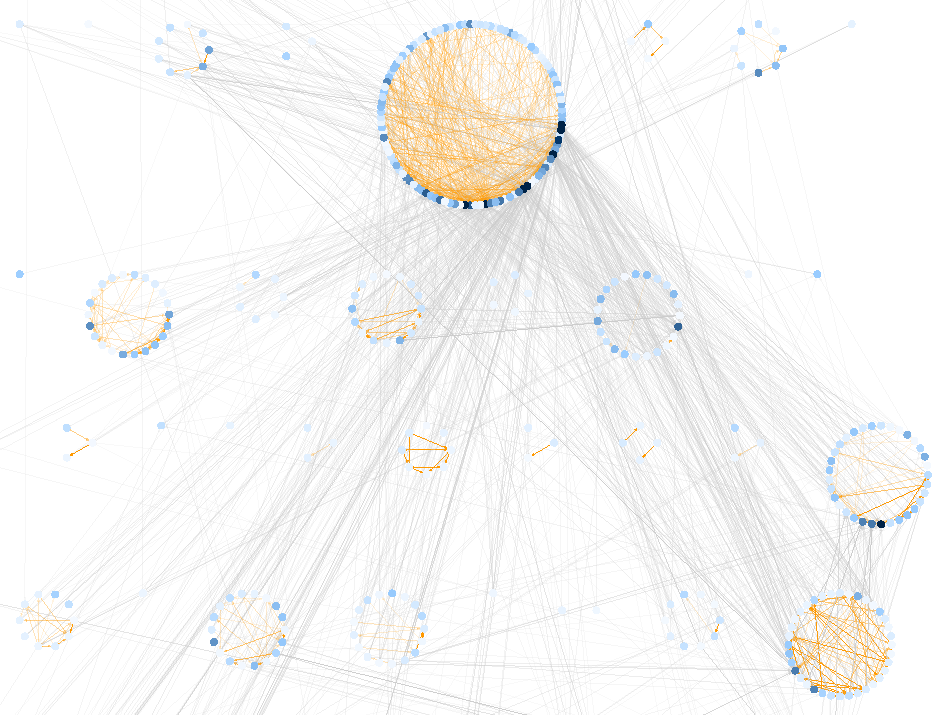
\includegraphics[width=\columnwidth]{Figs/final-overview.pdf}
    \caption{An example {\em Via} graph, showcasing enrollment
      patterns within different departments. Each ring is comprised of
      courses offered by one department.}
    \label{fig:overview}
\end{figure}

Tool users can zoom, and select particular courses or
departments. The selections can then be extracted as a separate
graph. These interactions are implemented by \textit{Cytoscape}, which
we use as the engine behind {\em Via}.

Cytoscape was developed to model biological systems and interactions
between cellular organisms. Yet the tool is well suited for
representing our academic pathway data.

Cytoscape uses a spring-embedder system for optimally spacing and
aggregating nodes, and additionally allows the tool operator to
cluster nodes by attributes \cite{Battista1994}. For our purposes, we
display courses within departments as ring structures. For example,
the large ring in Figure \ref{fig:overview} represents the Computer
Science department in a graph generated from enrollment data filtered
to include only CS majors. Each of the dots that comprise the
circumference of the ring is one course in that department. The
interior connecting arrows display the flow of students from one CS
course to another. Links between rings are enrollments of CS majors in
other departments' courses.

{\em Via} assigns unique colorings for both courses (nodes) and
enrollment probabilities (edges) to visualize course and
enrollment-level attributes. In all of the figures below, we color
edges between courses in the same department orange, and all edges
between courses in different departments grey. We further modulate the
opacity of an edge from course \textit{i} to course \textit{j} to
represent the conditional probability of taking course j after course
i. Finally, each node is colored in a blue-gradient, representing the
prior probability of a student enrolling in the respective course. For
example, a deep blue node would be a course that many students are
highly likely to enroll in during their undergraduate years.

Note that while a {\em Via} graph {\em aggregates} all students---no
single student's information is represented---we can choose to make
available to {\em Via} only students with certain characteristics. In
Figure~\ref{fig:overview} this attribute is {\em major}. We could as
easily construct such overviews that distinguish between, for example,
gender or minority status.

Beyond visualizations {\em Via} provides a second, more formal avenue
for analysis. As the tool's principle visual element is a graph, many
graph related mathematical approaches are available. These include
variations of centrality and betweenness, clustering, Page Rank, and
others. Applications below will exemplify the use of some such
methods.

\subsection{Student Stakeholders}
\label{sec:student-stakeholders}

\begin{figure}
    \centering
    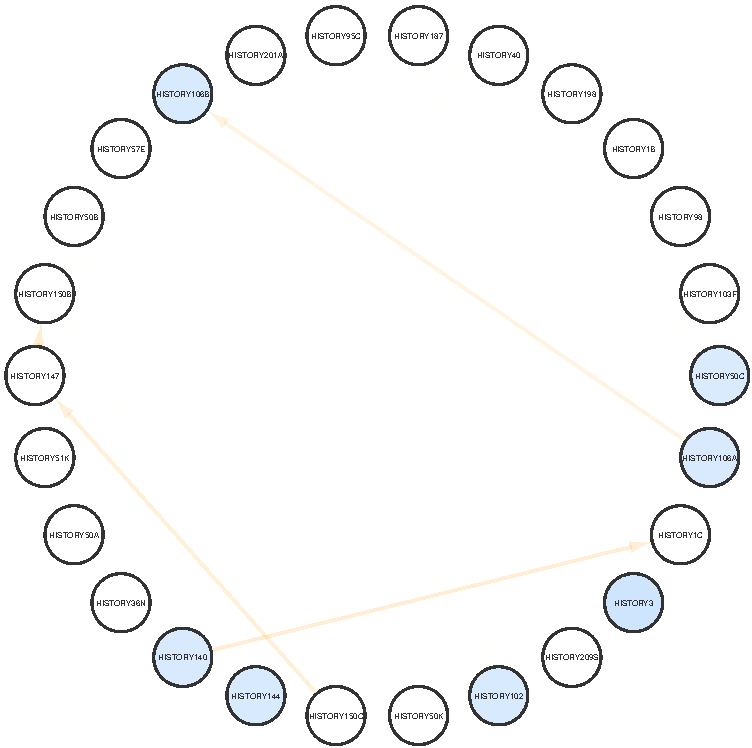
\includegraphics[width=0.55\columnwidth]{Figs/final-modularity-history.pdf}
    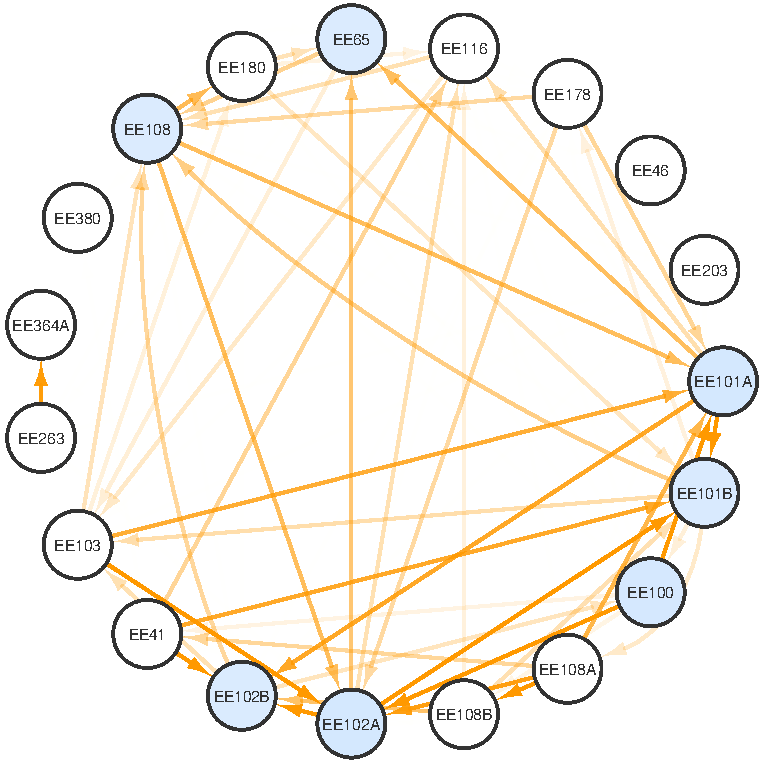
\includegraphics[width=0.44\columnwidth]{Figs/final-modularity-ee.pdf}
    \caption{A comparison between the student behavioral patterns in two departments---History (left) and Electrical Engineering (right)---from the years 2012-2016. Labels in the small circles are course names, such as ``\textsc{ee41}'' and ``\textsc{history198}''.}
    \label{fig:modularity}
\end{figure}

We next highlight two particular use cases. First, our visual modeling
of course sequences allows a student to identify which majors require
students to take courses from within primarily a certain department,
and which allow for more academic exploration across departments. We
can report this result both visually, by directly looking at the
intra-department orange arrows in a graph, and by calculating, the
{\em modularity} of certain departments. Modularity is another example
of how {\em Via}'s choice of graphs as building blocks enables the
application of well known mathematical tools. The metric represents
the connectivity of clusters within a graph, by calculating the
over-representation of edges among groups of nodes.

In Figure~\ref{fig:modularity}, we compare the interconnectivity of
the History, and Electric Engineering majors, limited to course
enrollments of one academic year apart.  Here we see that the
visualizations align with the modularity scores associated with
History (0.003) and Electrical Engineering (0.028). The higher the
modularity score the more a department is intra-connected. This effect
is caused by highly prescriptive requirement structures.

As a second use case, we illustrate how \textit{Via} can be leveraged
to discover the ''try-me'' courses. Departments offer such service courses for students
majoring in unrelated fields, but who are interested in exploring other
areas of study. {\em Via} enables quick discovery of such courses.

We find the ``try-me'' courses by creating a {\em Via} graph over
students of a single major. We then identify the most popular courses
within this generated graph that are not in that major. For instance,
by filtering on the History major, we observe that of the History
majors, nearly 28\% take \textsc{cs105} and 21\% take
\textsc{cs106a}. These trends are visualized through variations in
node coloration in Figure~\ref{fig:history-try-me}.

\begin{figure}[h]
    \centering
    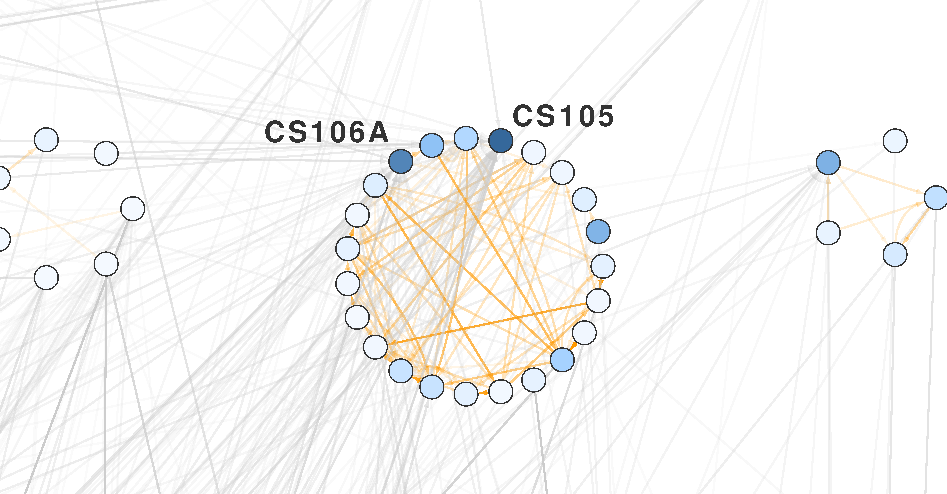
\includegraphics[width=.9\columnwidth]{Figs/final-history-try-me.pdf}
    \caption{A visualization of the most popular courses in the Computer Science department for History majors.}
    \label{fig:history-try-me}
\end{figure}

 Babad et al. have discovered that the primary reasons students decide
 to enroll in a particular course are the learning value of the class
 followed closely by the lecture style \cite{Babad2003}. Particularly
 difficult courses are avoided by students unless otherwise
 required. Our assessment of the recommended Computer Science
 ``try-me'' courses for History majors corroborates these
 results. Although \textsc{cs106a} is branded as the most enrolled
 introductory Computer Science course at the university from which we
 have acquired our dataset, \textsc{cs105} additionally presents
 itself as the Computer Science course for non-majors, and it is also
 known among students as less rigorous. Our \textit{Via} toolkit is
 thus able to offer a more personalized course discovery system for
 students of a particular major.
 

\subsection{Instructor Stakeholders}
\label{sec:instructor_stakeholders}

Instructors comprise a second group of stakeholders that can benefit from
the easy interpretability of our course sequence visualizations. It is
of particular interest to instructors to gain an overview of the sorts
of students enrolling in their courses, in order to customize
and improve lesson plans \cite{Leaver2002}.

\begin{figure}[h]
    \centering
    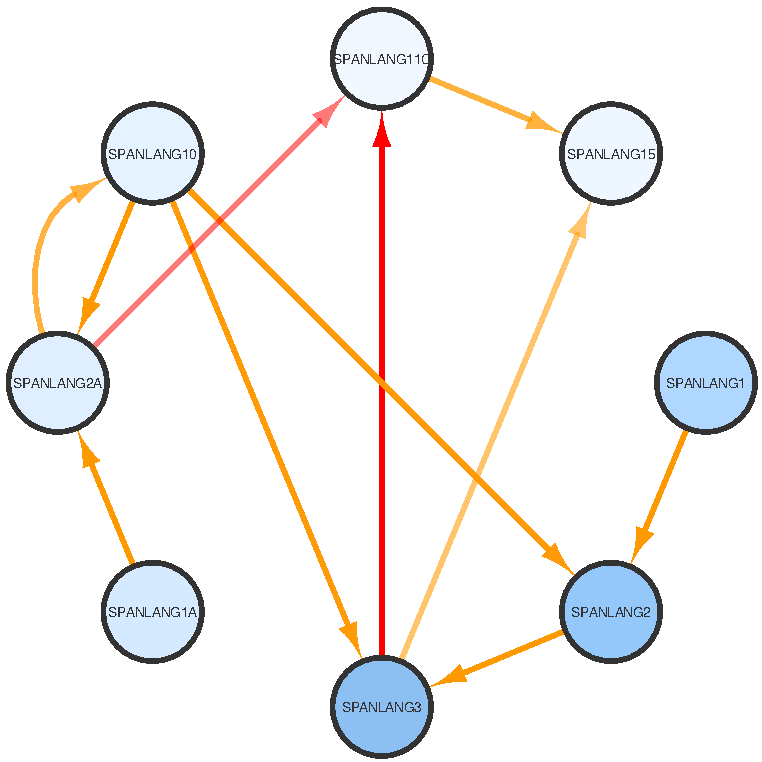
\includegraphics[width=0.4\columnwidth]{Figs/final-spanlang.pdf}  
    \caption{Relationships within the language department's Spanish course offerings from 2012-2016. We note that the probability that a student transitions from first to second year Spanish significantly increases if initially enrolled in the non-accelerated track.}
    \label{fig:spanlang}
\end{figure}

As an example, we show that it is possible to use the course probabilities associated with course-to-course interactions to study the background of students who take higher-level Spanish language classes. We do this by examining the conditional probability graph generated with
all enrollment data. Here we set our graph as sensitive only to
enrollments in course pairs within one year of each other in order to
capture delayed enrollment behaviors. We can thus interpret edge
weights as probability $p(i|j \text{ within the past year})$. In
Figure~\ref{fig:spanlang}, we examine the courses associated with the
V-structure colored in red---\textsc{spanlang3} (bottom),
\textsc{spanlang2a} (left), and \textsc{spanlang11c}
(top). \textsc{spanlang3} is the final term of the non-accelerated
offering of the first-year Spanish language sequence,
\textsc{spanlang2a} is the final term of the accelerated first-year
sequence (often taken by students with prior exposure to the language
through high school programs), and \textsc{spanlang11c} is the first
academic term of the second-year sequence.

From the visualization alone, it is evident that the relationship
between \textsc{spanlang3} and \textsc{spanlang11c} is stronger than
the relationship between \textsc{spanlang2a} and
\textsc{spanlang11c}. Indeed, the probability that a student enrolls
in \textsc{spanlang11c} within a year of completing \textsc{spanlang3}
is almost three times that of a student who enrolls in
\textsc{spanlang11c} after completing \textsc{spanlang2a}, with
$p(\textsc{spanlang11c}|\textsc{spanlang3}) = 0.038$ and
$p(\textsc{spanlang11c}|\textsc{spanlang2a}) = 0.013$.

This information is not readily gleaned from standard enrollment
figures. The number of students enrolled in \textsc{spanlang11c}
during the graph's time period is almost identical to enrollment in
\textsc{spanlang2a}. One might be erroneously tempted from these
numbers alone to conclude that most {\em 2a} students move on to
\textsc{spanlang11c}. Accounts based on raw enrollment are further
complicated by the observation that enrollment in \textsc{spanlang1-3}
is non-monotonic, first falling, then rising. The cause is
likely that students enroll in \textsc{spanlang3} directly.

A large contribution to \textsc{spanlang11c} beyond \textsc{spanlang3}
are in fact not {\em 2a} students, but students who are already
proficient enough to engage this culture-oriented class directly.

{\em Via} does not help an analysis of underlying reasons for
preferences between the two Spanish language sequences. However,
learning literature does suggest a reason. The observation is in
accordance with the research of Leaver \textit{et al.}, which details
the significance of varying teaching philosophies commonly seen in
foreign language classrooms at different language acquisition levels
\cite{Leaver2002}.

It is possible that the preference for the \textsc{spanlang1-3}
sequence is explained by the difference between instruction of
grammatical foundations in the university's introductory courses
compared to high school language programs.

We next describe details of how we construct the graphs in the above
applications from raw enrollment data.

\section{Methodology}
\label{sec:methodology}

\begin{figure}
    \centering
    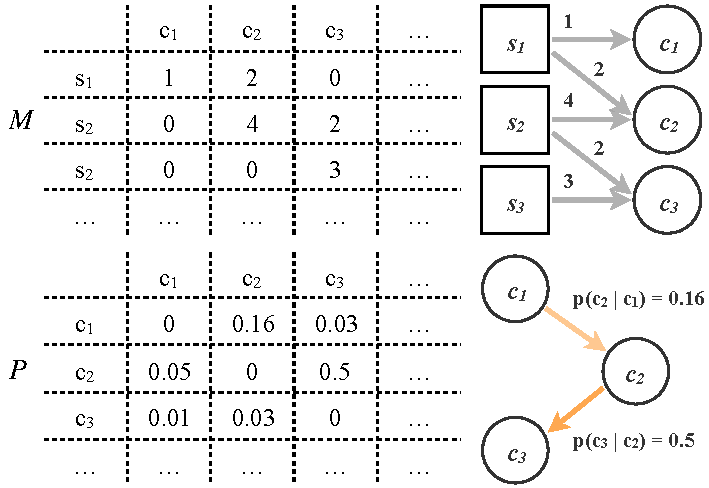
\includegraphics[width=\columnwidth]{Figs/final-simple.pdf}
    \caption{An overview of the projection created from enrollment
      data. Enrollment sequences are tallied and normalized to define
      a conditional probability of taking one course after
      another. Rows $s_i$ describe students, while columns $c_i$
      correspond to course offerings.}
    \label{fig:simple}
\end{figure}

Our first challenge is to build an expressive yet interpretable model
of course-to-course interactions that results in the graph-based
representation of academic pathways. The representation must support
the desired ability to discover student enrollment patterns over time
and enrollment interactions between departments.

We compile student-to-course enrollment information
into what we will call a course-to-course projection model, a network
that represents courses as nodes and course relationships as weighted
edges. 

Figure~\ref{fig:simple} illustrates the process. We begin with a
matrix $M$ representing student enrollment in courses over time. We
can interpret this matrix $M$ as the adjacency matrix of a bipartite,
labeled graph documenting the interaction of student nodes with course
nodes.  We end with a matrix $P$ that defines a projection of the
courses in $M$, where edge weights signify how strongly two courses
are linked. This projection can be visualized as a network such as the
one found in Figure~\ref{fig:overview}, which maps all course
interactions in a way that describes the aggregate behavior of student
enrollment patterns. In order to preserve the normal, sequential
nature of courses across academic years, we omit the Summer Period
from all experiments.

Combined with an existing graph manipulation kit---in our case Cytoscape
\cite{shannon2003cytoscape}---the graph described by $P$ serves as our
target toolkit for university stakeholders. We now show how we endow
the construction process of $P$ with flexibility that can tune the
resulting graph for visualizations that help answer a variety of
questions.

As per the overview above, the first step is to prepare a sequence
matrix. The second involves the calculation of the projection. The
following sections merely formalize the overview.

\subsection{Sequence Matrix Generation}
\label{sec:seq_martix}

{\em Via} receives data in the form of tabular student enrollment
records. The input to the projection algorithm is a matrix $M$ of
shape $(|S|, |C|)$, where $S$ is the set of all students and $C$ is
the set of all courses. A given entry $M_{ij}$ represents the time
when a student $i$ enrolls in some course $j$. For example, an entry
$M_{ij} = 1$ signifies that student $i$ enrolled in course $j$ during
their first academic term, generally quarter or semester. An entry
$M_{ij} = 0$ implies that $i$ never enrolled in $j$. This thus implies
that each row $m_i$ represents the entire course enrollment history of
some student $i$. We generate various forms of matrix $M$ from the raw
enrollment data by filtering on different student attributes. The
nature of the filter depends on the questions being asked. For
example, if we are only interested in those who majored in the Humanities, we would
limit $M$ to this student subset. Another filter one might apply at
this step is year of enrollment, if only that time slice is of
interest. The more filtering is applied to $M$ the faster the
subsequent processing, and visual interaction response.

Our data provides information on each enrollment's time, the enrolling
student's major at the time of enrollment, and the student's final
major. Depending on data availability, filters based on gender, status
as underrepresented minority, or college entrance scores could be
applied as well.

\subsection{Graph Projection}
\label{sec:graph_projection}
Next, given the sequence matrix $M$, we generate the matrix $P$ of
shape $(|C|, |C|)$. This matrix represents the adjacency matrix for a
one-mode projection of the bipartite network specified by matrix
$M$. We weight each edge in $P$ using conditional probabilities that
describe how likely one is to take one course given another
course. Thus, entry $P_{ij}$ represents the conditional probability of
taking course $j$ given that one has taken course $i$. $P$ aggregates
students, losing some information, but gaining the probability of moving from one course to another.

Matrix $P$ is thus a representation of how even non-adjacent course nodes in $M$ interact, based on the nature of student enrollment. We use this matrix $P$ as the basis of all calculations and visualizations. 
 The parameters for the conditional probabilities are fit based on counts determined in the calculation of intermediary matrix $\tilde{P}$ of shape $(|C|, |C|)$. We calculate each entry $\tilde{P}_{ij}$ by accumulating the occurrences of course $i$ taken at some point before course $j$ across all students in set $S$:
\begin{equation}
  \tilde{P}_{ij} = \sum_{s=1}^{|S|} \mathbbm{1}\{M_{si} - M_{sj} \geq 0\}* d(M_{si} - M_{sj})
\end{equation}
where $M_{si} - M_{sj}$ is the academic timestep delta (commonly
measured in semesters, or quarters) between a student $s$'s taking
course $i$ and course $j$. Function $d$ is a second point in the
visualization construction where flexibility is provided. The function
may be chosen to de-emphasize the connection between subsequent
courses.

For example, in an analysis of degree completion we may be interested
in cases when course offerings were taken as closely together as
possible. In contrast, when planning curricula we may wish simply to
learn the probabilities of two courses taken in sequence, even if
several academic terms apart.

Function $d$ may be chosen to be continuous or discrete.  For example,
the following choice attenuates the relationship between two courses
through an exponential decay over enrollment term distance:

\begin{equation}
  \tilde{P}_{ij} = \sum_{s=1}^{|S|} \mathbbm{1}\{M_{si} - M_{sj} \geq 0\}* \lambda^{M_{si} - M_{sj}}
\end{equation}
where, $\lambda$ is a constant that controls decay rate. Intuitively, this type of function gives more weight to close course-pair enrollments than temporally distant course-pair enrollments.

Alternatively, we may choose a function $d$ that tallies a
relationship between two courses only when course $j$ immediately
follows course $i$. In the following example, elapsed time between two
courses beyond one term would sever the relationship:
\begin{equation}
d = \begin{cases} 
      1, & M_{si} - M_{sj} = 1 \\
      0, & M_{si} - M_{sj} > 1 
    \end{cases}
\end{equation}
More elaborate discrete functions could amplify course relationships of
particular time distances.

Using $\tilde{P}$, we calculate the final projection matrix $P$. In some experiments, we set $P = \tilde{P}$, in order to gain access to a raw count projection matrix. In other experiments, we set $P$ to be a matrix of conditional probabilities between courses. In this case, each entry $P_{ij}$ is a conditional probability $p(j|i)$ whose parameters are computed using the following closed form expression:
\begin{equation}
    P_{ij} = p(j|i) = \frac{\tilde{P}_{ij}}{\sum_{s=1}^{|S|}\mathbbm{1}\{M_{si} > 0\}}
\end{equation}
$P_{ij}$ thus represents the proportion of students who take the
course sequence: course $i$ followed by $j$ out of the total number of
students who take course $i$ at any point. One may note that this
bears a resemblance to a Bayesian Network; however, we make the
assumption that the process of transitioning from course node to
course node is Markovian in nature. This eases implementation but
precludes our model from being a true Bayesian Network due to the
emergence of cycles.
%In our domain cycles should be allowed in the model. They describe 

In the following section we describe how we combine the projection
matrix with an existing graph visualization tool. For simplicity we
choose the timestep delta function $d$ to be discrete, although we
can alter the nature of the function for different examples.


%% \subsection{Administrator Stakeholders}
\label{sec:administrative_stakeholders}

With the underlying data structures explained, it is now clear how
{\em Via} builds special subgraphs by filtering early, when the
student level information is still available. The filtering occurs as
matrix $M$ is constructed. Similarly, the discount function is used to
control how closely together we wish enrollments to have occurred in
time. The following application takes advantage of the adjacency
matrix itself, not explicitly creating a graph.

Our model provides an intuitive medium for understanding
department-wide dynamics across varying student
demographics. Administrators in charge of course resource allocation
may be interested in the enrollment patterns of students as they move
through a department's course offerings. We provide two use cases to
illustrate how \textit{Via} can be leveraged to derive insights into
the structure of courses within departments.

First, we study which classes tend to guide a student into a certain
department. We report the top 10 classes within a department that,
once taken by a student, have the highest average number of subsequent
enrollments within the same department. In
Figure~\ref{fig:persistence} we show the student persistence within a

\begin{figure*}[h!]
    \centering
    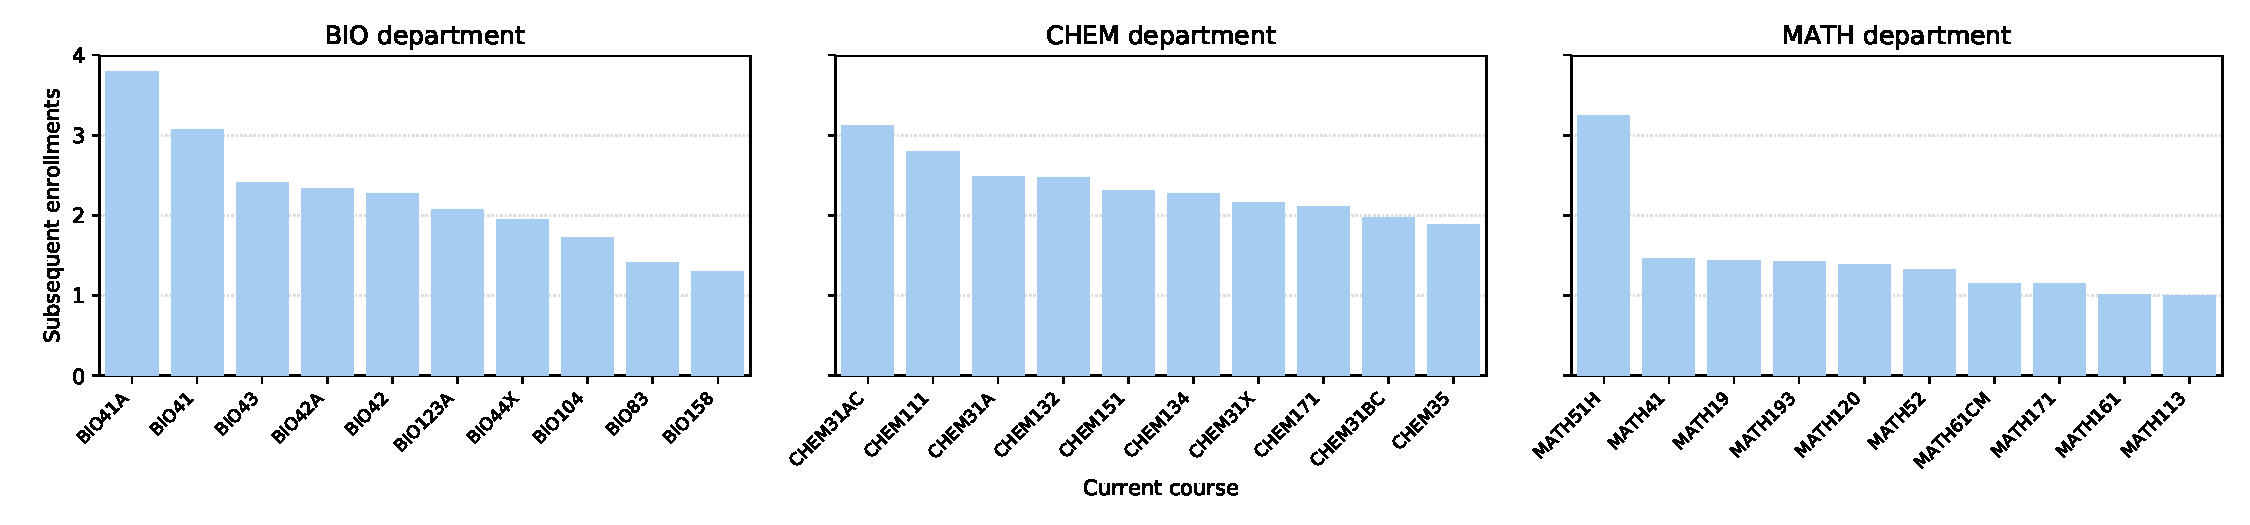
\includegraphics[width=18cm]{Figs/final-persistence.pdf}
    \caption{Student persistence metrics in Biology, Chemistry and
      Mathematics. The support courses for the biology and chemistry
      departments' introductory courses, \textsc{bio41a} and \textsc{chem31ac},
      respectively, lead to higher subsequent enrollment rates within
      the respective departments.}
    \label{fig:persistence}
\end{figure*}

department using a raw count projection model with discrete discount
function $d$ that captured all non-co-enrollment relationships between
courses from 2014-2018.  This ``persistence within a department''
metric can be computed for a given class $i$ in a department $x$ by
finding the out-degree of the class node and then dividing by the
total number of students who enrolled in class $i$. This method is
equivalent to finding the expected number of courses taken within
department $x$ after enrollment in class $i$. Observe that this is
robust to a course's discontinuation across academic years due to the
conditions under which the ratio is calculated. Here we measure the
average number of courses taken within a department after having
enrolled in a given course. Within the Biology and Chemistry
departments, we recover the insight that the 1-unit companion courses
to the introductory courses (\textsc{bio41a} and \textsc{chem31ac} for
Biology and Chemistry, respectively) increased student
persistence. Intuitively, this observation indicates that enrollment
in these courses led to an overall increase in the number of courses
taken within the department, on average. We contrast this with the
Math department. Students who enrolled in the most courses offered
within the Math department were those who enrolled in the first course
of the honors multivariable mathematics sequence,
\textsc{math51h}. This observation can be explained by the fact that
the classes in the primary introductory course sequence in the Math
department (\textsc{math51}, \textsc{math52}, \textsc{math53}) often
serve as prerequisite courses for classes in other departments in
engineering and social sciences. Enrolling in the honors-level
mathematics sequence perhaps indicates a given student's higher
intrinsic inclination to the subject matter.

\section{Advanced Applications}
\label{sec:advanced}

With the underlying data structures explained, it is now clear how
{\em Via} builds special subgraphs by filtering early, when the
student level information is still available. The filtering occurs as
matrix $M$ is constructed. Similarly, the discount function is used to
control how closely together we wish enrollments to have occurred in
time. Several of the applications above used these techniques.

We next introduce applications that rely on the graph data structure
less as a visualization method. Instead curriculum insights are gained
from mathematical analyses of the graph that is described by the
projection matrix $P$.\footnote{At the time of this writing we have not
  yet provided access to these methods through {\em Via}'s user
  interface.}





% \subsection{Evolution of Program Flexibility}
\label{sec:course_pref_evolution}

We begin by showing how {\em Via} recovers high-level, university-wide
trends that have been independently observed in the literature.

We determine the overall {\em flexibility} of departments and their
programs during varying historic time periods. High flexibility means
high ability of students in majors outside the program to include the
program's courses in their curriculum. The measure is thus
complementary to the requirements analysis of
Section~\secref{sec:student-stakeholders} (Figure~\ref{fig:modularity}).

To compute department flexibility for our specific university over
time we use {\em Via} to create separate graphs for generations of
students, separated by their orientation towards engineering, versus
the humanities and social sciences.

We use raw counts of consecutive course enrollments from term to term
to define edge weights between courses. The PageRank execution then
turns those raw counts into transition probabilities.

\begin{figure}
    \centering
    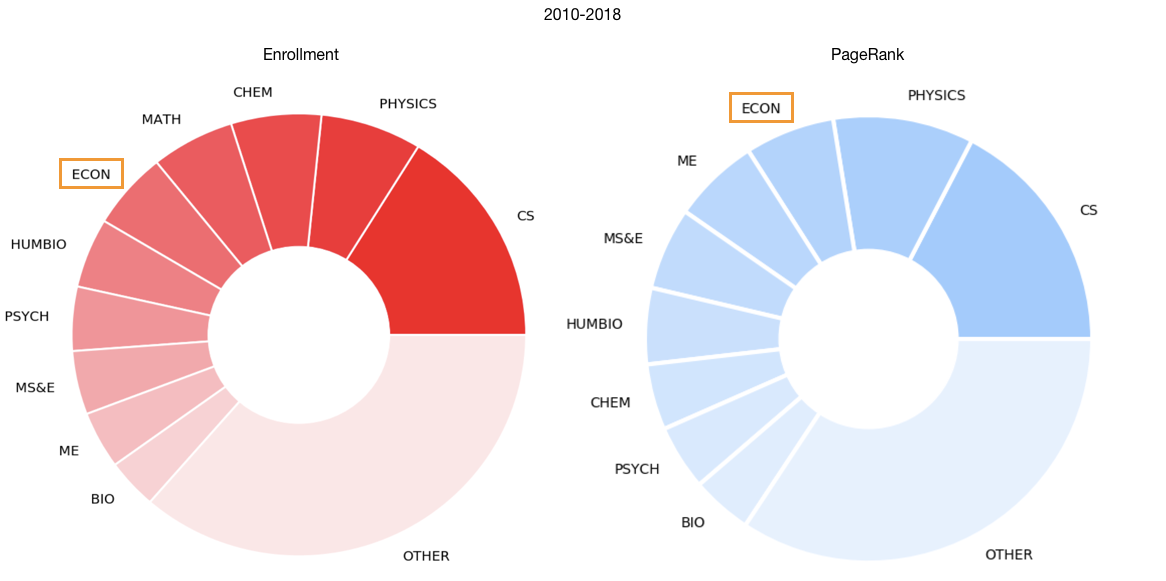
\includegraphics[width=\columnwidth]{Figs/final-enrollment-vs-pagerank.png}
    \caption{Caption}
    \label{fig:my_label}
\end{figure}


\begin{figure}
    \centering
    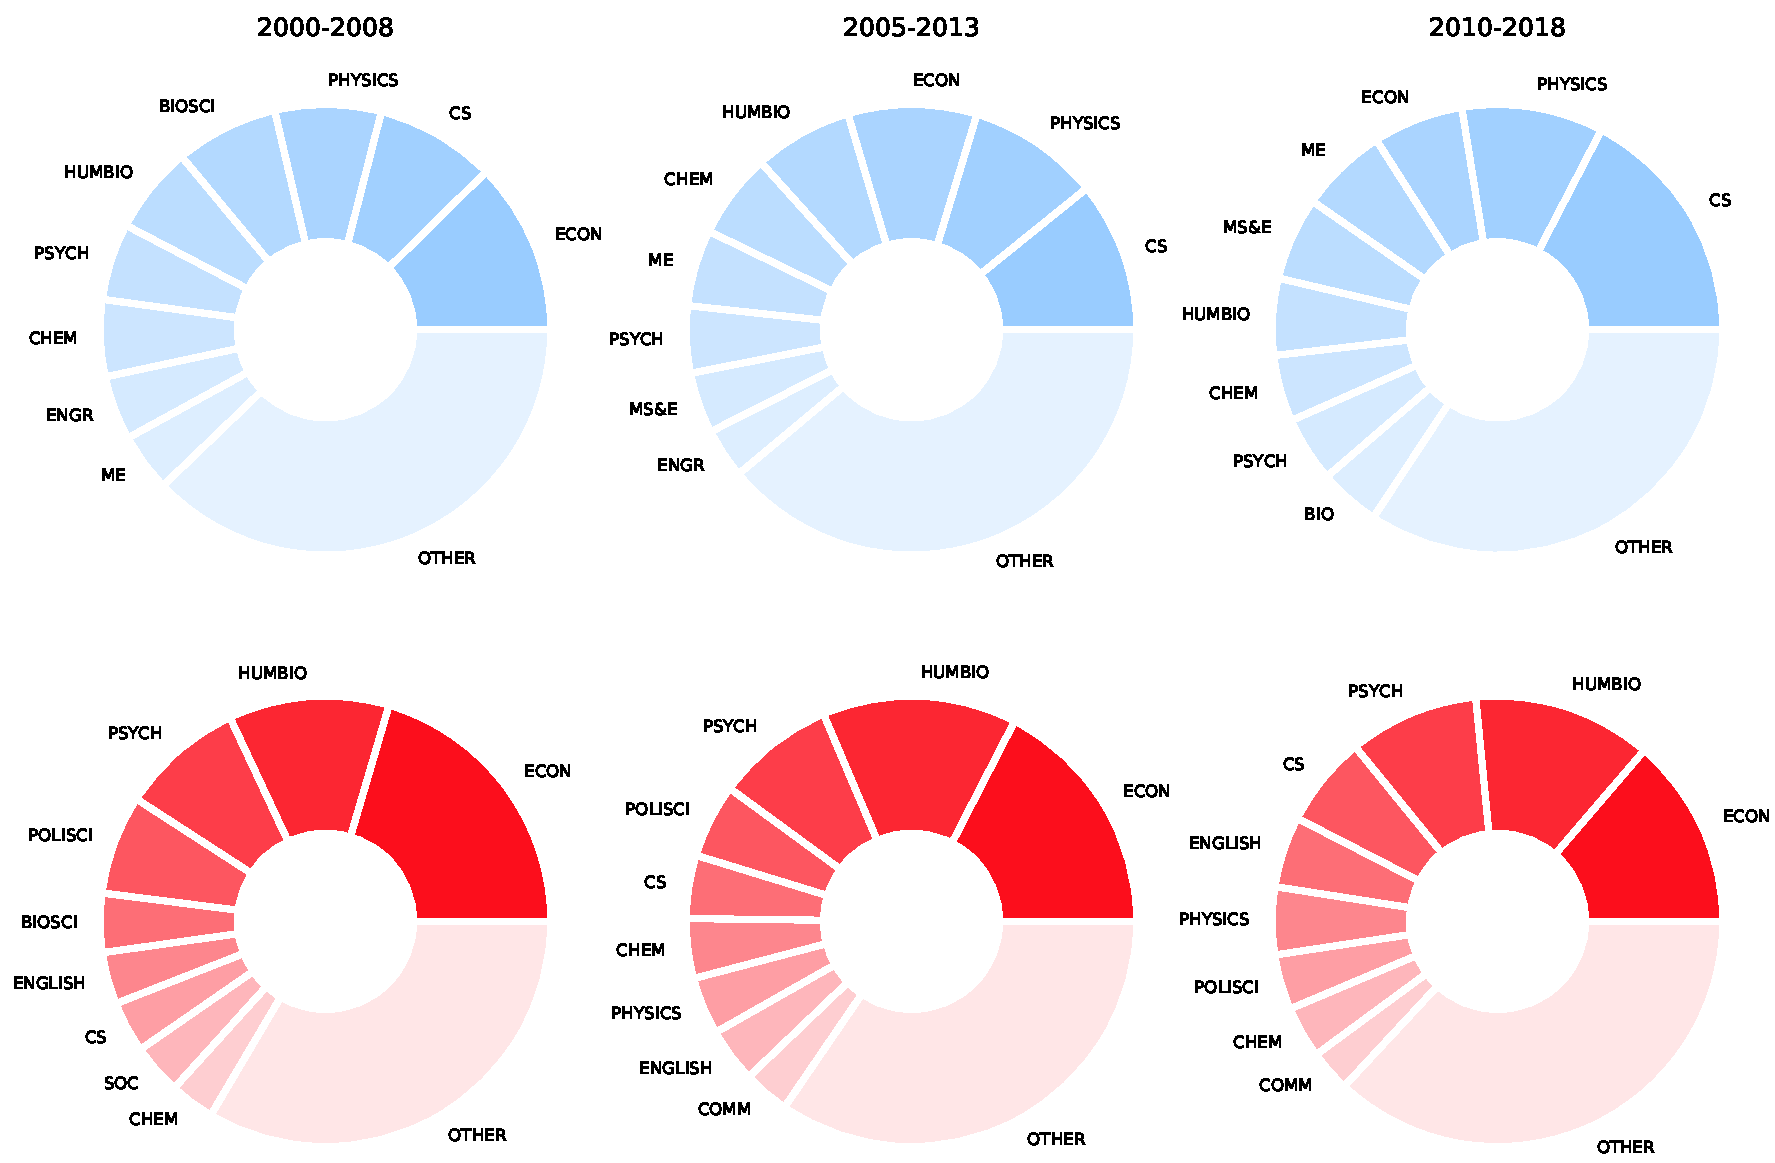
\includegraphics[width=\columnwidth]{Figs/final-evolution.pdf}
    \caption{A comparison over time of PageRank values by department
      in both the entire undergraduate network (top row) and the
      undergraduate network filtered on students who earned a
      Bachelor's of Arts (BA) degree (bottom row).}
    \label{fig:evolution}
\end{figure}

Figure~\ref{fig:evolution} shows the result.

We can interpret the final results as follows: for a given department
$D$ with PageRank score $X$, starting at a random course, and
selecting successors according to successor probability will land
students in $D$ $(X * 100)$\% of the time. Thus, the percentages in
Figure~\ref{fig:evolution} signal the ease with which a department's
courses are available without following a prescribed path.

More generally, we can interpret the relative size of the departments
in Figure~\ref{fig:evolution} as the flexibility of departments across
the different disciplines at the university throughout any time period
in an undergraduate's career.


%% This quantity has an inverse
%% relationship with the activation energy required to begin taking
%% courses in a given department.

%% In this case a department's high PageRank score would indicate a
%% relative ease of entering and taking a course within a particular
%% department.
While closely linked, flexibility differs from metrics of student
composition and enrollments. For example, we see that missing from the
2010-2018 undergraduate results is the mathematics department, despite
it ranking 4th in raw number of enrollments during the given
timeframe. This is likely because students become much less likely to
enroll in math courses after fulfilling the requirement (commonly
during their freshman year), whereas many students enroll in many of
the popular courses in the CS, ECON, and ME departments throughout
their undergraduate career, perhaps because these subjects are less
dependent on knowledge acquired---or not acquired---during the final
years of high school.

We observe that between 2000 and 2018, the PageRank score of the
Computer Science department has increased. This observation applies in
general to all degree-seeking students and to the BA-seeking
students.

Another point to note is a general decrease in accessing economics
courses, but a noticeable uptick in the number of classes taken in
Management Sciences and Engineering (MS\&E). These two trends are
strongly correlated, as the material of MS\&E seeks to combine
economics and finance with computer science and statistics.




Our results are in harmony with observations made by education researchers. Over the past 20 years the proportion of students majoring in STEM, and particularly computer science has varied greatly \cite{ComputingResearchAssociation2017}. Introductory, mid-level and upper-level computer science courses have all shown a demonstrable increase upwards of 150\% of student enrollment between 2000 and 2017. Driving student's decisions to enroll in more technical courses is primarily the greater monetary compensation that these majors promise at the workplace \cite{Downey2007}. Interestingly, however, while the total amount of classes taken within Computer Science has risen noticeably, we do not observe that the total amount of student majors in Computer Science has increased at the same rate. Rather between 2000 and 2010 the number of Computer Science majors showed an uptick of 33\%. However, between 2010 and 2018 the percent increase of Computer Science majors drops to 5.8\%. This finding is more generally in line with the observed trend that the Computer Science major has not experienced a constant exponential increase in popularity. Rather, 2005 was one of the years with the lowest rates of students who self-reported interest in majoring in Computer Science when entering college \cite{Patterson2005}. Between 2000 and 2008 it was, in fact, economics and business-related courses that remained one of the most popular majors of study nation wide \cite{NationalCenterforEducation2018}. Overall, our quantitative analysis is able to corroborate much of the education research regarding course enrollment patterns over the past 20 years. We stress that the methodology used to generate these results is not dependent on the source of data, but is rather facilitated by the graphical modeling of student course enrollments that \textit{Via} enables. In addition, the incorporation of filtering mechanisms beyond time, such as student demographics, would allow for more fine grained understanding of course accessibility based on enrollment data alone.

\subsection{Course Discovery}
An important use case of our model is predicting prerequisites for
courses which have no explicitly listed required classes. Because {\em
  Via} models the interactions between courses as a graph, we can
leverage the {\em PageRank} algorithm for this task
\cite{Page1999}. PageRank measures the relative importance between nodes in a graph by conducting random walks through a network.

The algorithm is best known for its application in Web search. In the
curriculum domain, PageRank models many generations of students moving
through courses. The model provides probabilities of courses that
students with a given course history will take subsequently in their
college careers: it illuminates pathways based on prior
behavior. The random walk in this context is an imaginary new student
who is enrolled in a {\em seed course}. From there the student
randomly enrolls in successor courses, guided by the probabilities in
the projection matrix, until the student reaches a pre-determined
target course $C$.

Importantly, PageRank goes beyond counting enrollments---the course
node incidence of links into $C$. The algorithm mirrors the
probability that a student arrives at $C$ from other courses, which
might be topically distant. The algorithm thus takes into account path
lengths, not just the immediate enrollment history prior to $C$.

We demonstrate two examples of how the PageRank algorithm grants us
insights into implicit prerequisite relationships that exist between
courses.

{\bf Which math alternative to choose:} For the first example, let us imagine a student who hopes to take \textsc{cs200}, a course that covers a broad introduction to Machine Learning methods.  The course is offered by
the Computer Science department in the School of Engineering.

In order to take this class, students are required to understand
matrix calculus and linear algebra. The two introductory mathematics
courses offered to first-year undergraduates are \textsc{engr1} and
\textsc{math1}. Among these two courses, \textsc{engr1} is offered by the School of Engineering, and is branded as an introductory mathematics course with an engineering focus. Based on the course catalog alone, \textsc{engr1} is ostensibly the introductory math course to take if one is interested in engineering. \textsc{math1} is offered as the more general introductory math course, often taken by students from outside the School of Engineering. Taking \textsc{engr1} over \textsc{math1} would seem to be a reasonable choice for a student seeking to take \textsc{cs200}. 

Yet aggregated data on student behavior suggests otherwise. Running PageRank twice, once with the seed course set as \textsc{math1} and once with \textsc{engr1}, we find that a student is more likely to complete
\textsc{cs200} after completing \textsc{math1}. Contrary to our premonition, this result indicates a stronger sequential relationship
between \textsc{math1} and \textsc{cs200} than between \textsc{engr1} and \textsc{cs200}. We suspect that students, instructors, and administrators all might benefit from illuminations of this sort.

One might argue that such insights could be gleaned from simple
database queries over enrollment data to show that \textsc{math1} and \textsc{cs200} have a higher joint enrollment count than \textsc{engr1} and \textsc{cs200}. When analyses are even mildly more complex than that, however, the approach becomes intractable.

Consider the case in which we are conditioning on more than
one course---say a student's entire course history. The intersection
of students with this precise set of courses is small, perhaps too
small to derive any meaningful statistical analysis of future
behavior. In its use of random walks, PageRank gives us a simple, yet
efficient method of approximating common student behaviors given a set
of courses already taken. The following illustrates this point.


{\bf De facto Prerequisites:} Consider the common scenario in
which a first-year undergraduate finds an upper
level course with few or no listed prerequisites. In the following
example the course is \textsc{polisci114d}, {\em Democracy, Development, and
  the Rule of Law}. Its student composition skews heavily towards
third- and fourth- year undergraduates and graduate students. The
student wishes to find a course that will prepare her for this upper
level offering.

We seed the PageRank algorithm with the four courses that the student
has already taken. We set \textsc{polisci114d} to be the target of all random
walks (enrollments).

\begin{figure}
    \centering
    \noindent\fbox{%
    \parbox{\columnwidth}{%
        \textbf{POLISCI~131L: Modern Political Thought: Machiavelli to Marx and Mill}
        This course offers an introduction to the history of Western political thought from the late fifteenth through the nineteenth centuries. We will consider the development of ideas like individual rights, government by consent, and the protection of private property. We will also explore the ways in which these ideas continue to animate contemporary political debates. Thinkers covered will include: Niccolò Machiavelli, Thomas Hobbes, John Locke, Jean-Jacques Rousseau, Edmund Burke, John Stuart Mill, and Karl Marx.
        }%
    }
    \noindent\fbox{%
    \parbox{\columnwidth}{\textbf{POLISCI~114D: Democracy,
        Development, and the Rule of Law} This course explores the
      different dimensions of development---economic, social, and
      political---as well as the way that modern institutions (the
      state, rule of law, and democratic accountability) developed and
      interacted with other factors across different societies around
      the world.  } }
    \caption{Descriptions of the top intermediary course candidate,
      POLISCI~131L, and the target course, POLISCI~114D.}
    \label{fig:pr-course-descriptions}
\end{figure}

We then iterate through the course catalog: at each iteration, we take
one course as the candidate for best preparatory course. We append it
to the initial four-class seed, 'pretending' the student had taken
this course. We then run PageRank from the augmented seed set, and
note the PageRank score of the target course. Upon loop termination,
we select as good candidates the top $k$ courses that led to the
highest target course PageRank.  See
Figure~\ref{fig:course-recommendation-algorithm} for a pseudo-code
implementation of the algorithm for $k=1$.

In this example, the top candidate course discovered by our algorithm
is \textsc{polisci131l}, {\em Modern Political Thought: Machiavelli to Marx
  and Mill}. The catalog excerpts in Figure
\ref{fig:pr-course-descriptions} confirm that this course is a good
choice. Unlike the target course, 71\% of students take the course in
their first two years. This example shows how PageRank reaches beyond
analyses derived solely from enrollment data queries.

%% We can immediately see a relationship between the two
%% courses in their official catalog descriptions (full texts found in
%% Figure \ref{fig:pr-course-descriptions}): the candidate course focuses
%% on foundational concepts such as ``individual rights, government by
%% consent, and the protection of private property,'' and the target
%% course focuses on ``the way that modern institutions (the state, rule
%% of law, and democratic accountability) developed and interacted with
%% other factors across different societies around the world.''

\lstset{language=Python}          % Set your language (you can change the language for each code-block optionally)

\begin{figure}
    \begin{lstlisting}[frame=single] 
let max_score = 0
let best_course = None 

let initial_classes = [ 'POLISCI1',
                        'STATS60',
                        'POLISCI102',
                        'POLISCI103']
                        
let target_class = 'POLISCI114D'

for course in courses:
    if course is in initial_classes:
        continue
    else:
        initial_classes.append(course)
        score = page_rank(initial_classes
                          target_class)
        if score > max_score:
            max_score = score
            best_course = course
        
        initial_classes.remove(course)

return (max_score, best_course)
\end{lstlisting}
\caption{Pseudo-code implementation of a course candidate search algorithm based on PageRank scores.}
\label{fig:course-recommendation-algorithm}
\end{figure}

The algorithm features several tunable parameters. For example, a
student can weigh their seed set such that some courses have higher
influence over the final decision than others. A student who may have
recently switched majors may want their queries to skew more heavily
towards their new major. In these cases, a student may decide to weigh
their most recent courses more heavily than others. Students can also
constrain the candidate course set to courses they have already
researched, as opposed to performing a search over the entire course
catalog.

\subsection{Curricular Course Roles}
\label{sec:rolx}
Courses often play particular roles in their department, or across a
university. We already mentioned service courses that provide non
majors with a taste of the department's discipline. Personnel within a
department generally understand these roles. But department outsiders
do not possess such knowledge. Researchers such as education or
sociology scholars studying universities and colleges other than their
own have even less access to role information.

We illustrate here how {\em Via} can recover course ``roles.'' The
application of more sophisticated algorithms rooted in graph theory
allows {\em Via} users to detect both roles and communities within
course networks. To this end we applied a {\em RolX}
\cite{Henderson2012} analysis, which requires enrollment data
alone. Intuitively, the analysis attempts to identify sets of course
nodes across a graph that are similar in enrollment history, and
position in students' pathways. The algorithm then attempts to
identify families of such courses, analogously to how {\em k-means}
defines clusters. As with clustering, RolX does not provide semantics
for discovered clusters. Those must be provided by human
interpretation.

Concretely in terms of graph analysis concepts, we represent each
course as a six-dimensional vector of its:
\squishlist  % itemize with less space between the bullets.
  \item In-degree.
  \item Out-degree.
  \item Betweenness centrality: Sum of the fraction of all course pairs
    whose shortest enrollment paths pass through the course node.
  \item Closeness centrality: closeness to all other courses enrolled
    in after the course.
  \item Closeness centrality, reversed: closeness to all other courses
    enrolled in before the course.
  \item PageRank
\squishend
The {\em RolX} analysis clusters these vectors, resulting in three
course roles. 

Figure~\ref{fig:rolxOverview} shows a layout of courses by role.
\begin{figure}
    \centering
    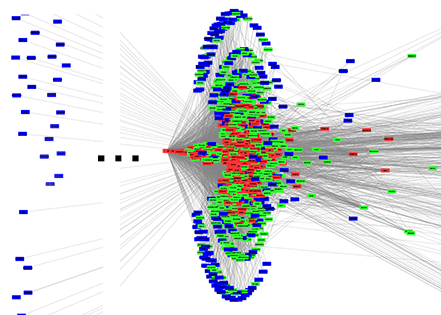
\includegraphics{Figs/rolxOverviewCropped2PhotoshopCroppedDoctoredWhite.png}
    \caption{Overview of courses that fill one of three discovered
      {\em RolX} roles. Red: introductory; green: intermediate; blue:
      enrichment. (Elision and cropping to fit publication.)}
    \label{fig:rolxOverview}
\end{figure}
We manually---therefore subjectively---examined catalog descriptions
of courses in the three roles. The red courses are introductory into
their department's fields, such as {\em Introductory Fluids
  Engineering}. The green courses are intermediate offerings, which
would usually be taken by majors in the field. Another example from
this roles is {\em Computer Vision: From 3D Reconstruction to
  Recognition}. The final role, blue, comprises enrichment courses of
general interest and accessibility, and seminars.

In {\em Via} the roles turn into course attributes, by which we can
filter, color, and layout courses and
enrollments. Figure~\ref{fig:rolxIntroCourses} is the result of extracting
the subgraph in the center of Figure~\ref{fig:rolxOverview},
filtering to include only introductory-role courses, coloring course
nodes by discipline, and automatically having them laid out in
circles.
\begin{figure*}
    \centering
    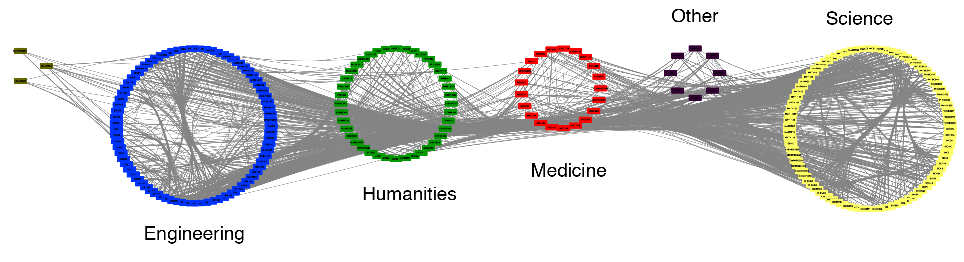
\includegraphics[width=\textwidth]{Figs/rolxIntroCoursesByDepartmentCropped.pdf}
    \caption{Introductory courses available in different disciplines.}
    \label{fig:rolxIntroCourses}
\end{figure*}
The task of finding introductory courses in the sciences now simply
involves clicking on any of the yellow nodes to see the course name,
or zooming in on the Science circle to see all the course name labels.

A final task that exploits roles is creation of an overview that shows
how many courses of each role the departments of the university
contribute to the curriculum. Figure~\ref{fig:rolxCircles} shows the
result.
\begin{figure}
    \centering
    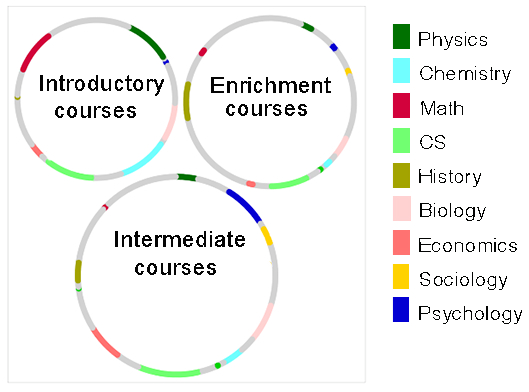
\includegraphics{Figs/rolxRingsCroppedLegendOutside.pdf}
    \caption{Which department offers courses in each of the three
      roles? (Legend created outside of tool.)
    }
    \label{fig:rolxCircles}
\end{figure}
Each circle's rim contains all courses that serve one role. The
circles were automatically constructed by requesting a circular layout
of all courses by the course role attribute. Courses of a particular
department were then selected by specifying that the names of courses
begin with, for example, {\em physics}. This action selected segments
of each role ring that was comprised of physics courses. The final
action was then to assign a color to those courses. The dark green
segments of the circles in the Figure therefore indicate physics
courses.


\section{Conclusion and Future Work}
\label{sec:conclusion}
We have described and demonstrated our {\em Via} toolkit, which is
constructed atop a new approach for visualizing and interpreting
transcript enrollment data. Such data are available at every major
US university. {\em Via} allows stakeholders as diverse as
students, instructors, and administrators to understand aggregate
student behavior over time. Using graph visualization and graph
theoretic computation in concert we have presented several {\em Via}
use cases.

We explained the process through which standard enrollment data can be
transformed into graph structures that may be tuned to particular
investigative goals. This flexibility arises both during graph
construction, and during interactive manipulation of the
graphs. We deploy the existing tool Cytoscape for such
manipulations, but other tools may be just as appropriate, once graphs
are constructed through the algorithm we have presented.

We will continue our exploration by investigating networks with
multiple node types: one to represent students, another to model
courses. The answers to other types of questions will be found through
this different family of graphs. 

We further plan to extend {\em Via} to include support for simulations
and what-if analyses. Further effort will also need to be invested
into making the graph construction process easy to use. 

Many questions may be answered by skillful SQL queries over university
datasets. But these approaches often fall short when questions are
not yet clearly defined, and relatively large amounts of data need to
be shaped and reshaped to discover patterns. As postsecondary
education is increasingly held accountable for performance, a deep
understanding of such patterns and trends over time will be
required. We have presented a fresh step toward such capability.


% BALANCE COLUMNS
\balance{}
% REFERENCES FORMAT
% References must be the same font size as other body text.
\bibliographystyle{SIGCHI-Reference-Format}
{\small\bibliography{coursePrecedence}}

\end{document}

%%% Local Variables:
%%% mode: latex
%%% TeX-master: t
%%% End:
https://www.overleaf.com/project/5ca66da716331457dbbdbcc8https://whttps://www.overleaf.com/project/5ca66da716331457dbbdbcc8ww.overleaf.com/project/5ca66da716331457dbbdbcc8
